\chapter{実験結果}
\section{一列配列イオン}
\subsection{イオン捕獲位置のdc電圧依存性}
dc電圧の変化に伴う単一イオンの捕獲位置の変位とシミュレーション結果におけるイオンの捕獲位置の比較を行った.シミュレーションはMathematicaで行い,プレーナートラップ上でx=0におけるSecularポテンシャルの最小値をイオンの捕獲位置とした.実験を行うにあたり,\Tb{dc_string}に示すdc電圧セットにおいて$V_{\rm End1}, \ V_{\rm End3}$に印加する電圧を$0.54 \sim 2.84$Vまで0.1Vずつ変化させたときのイオンの捕獲位置の記録を行った.\Tb{dc_string}の条件でのイオン捕獲位置を基準位置とし,End1,End3の電極に印加するdc電圧を変化させたときのイオン捕獲画像を\Fig{displacement_End13}に示す.
\begin{figure}[h]
	\begin{center}
		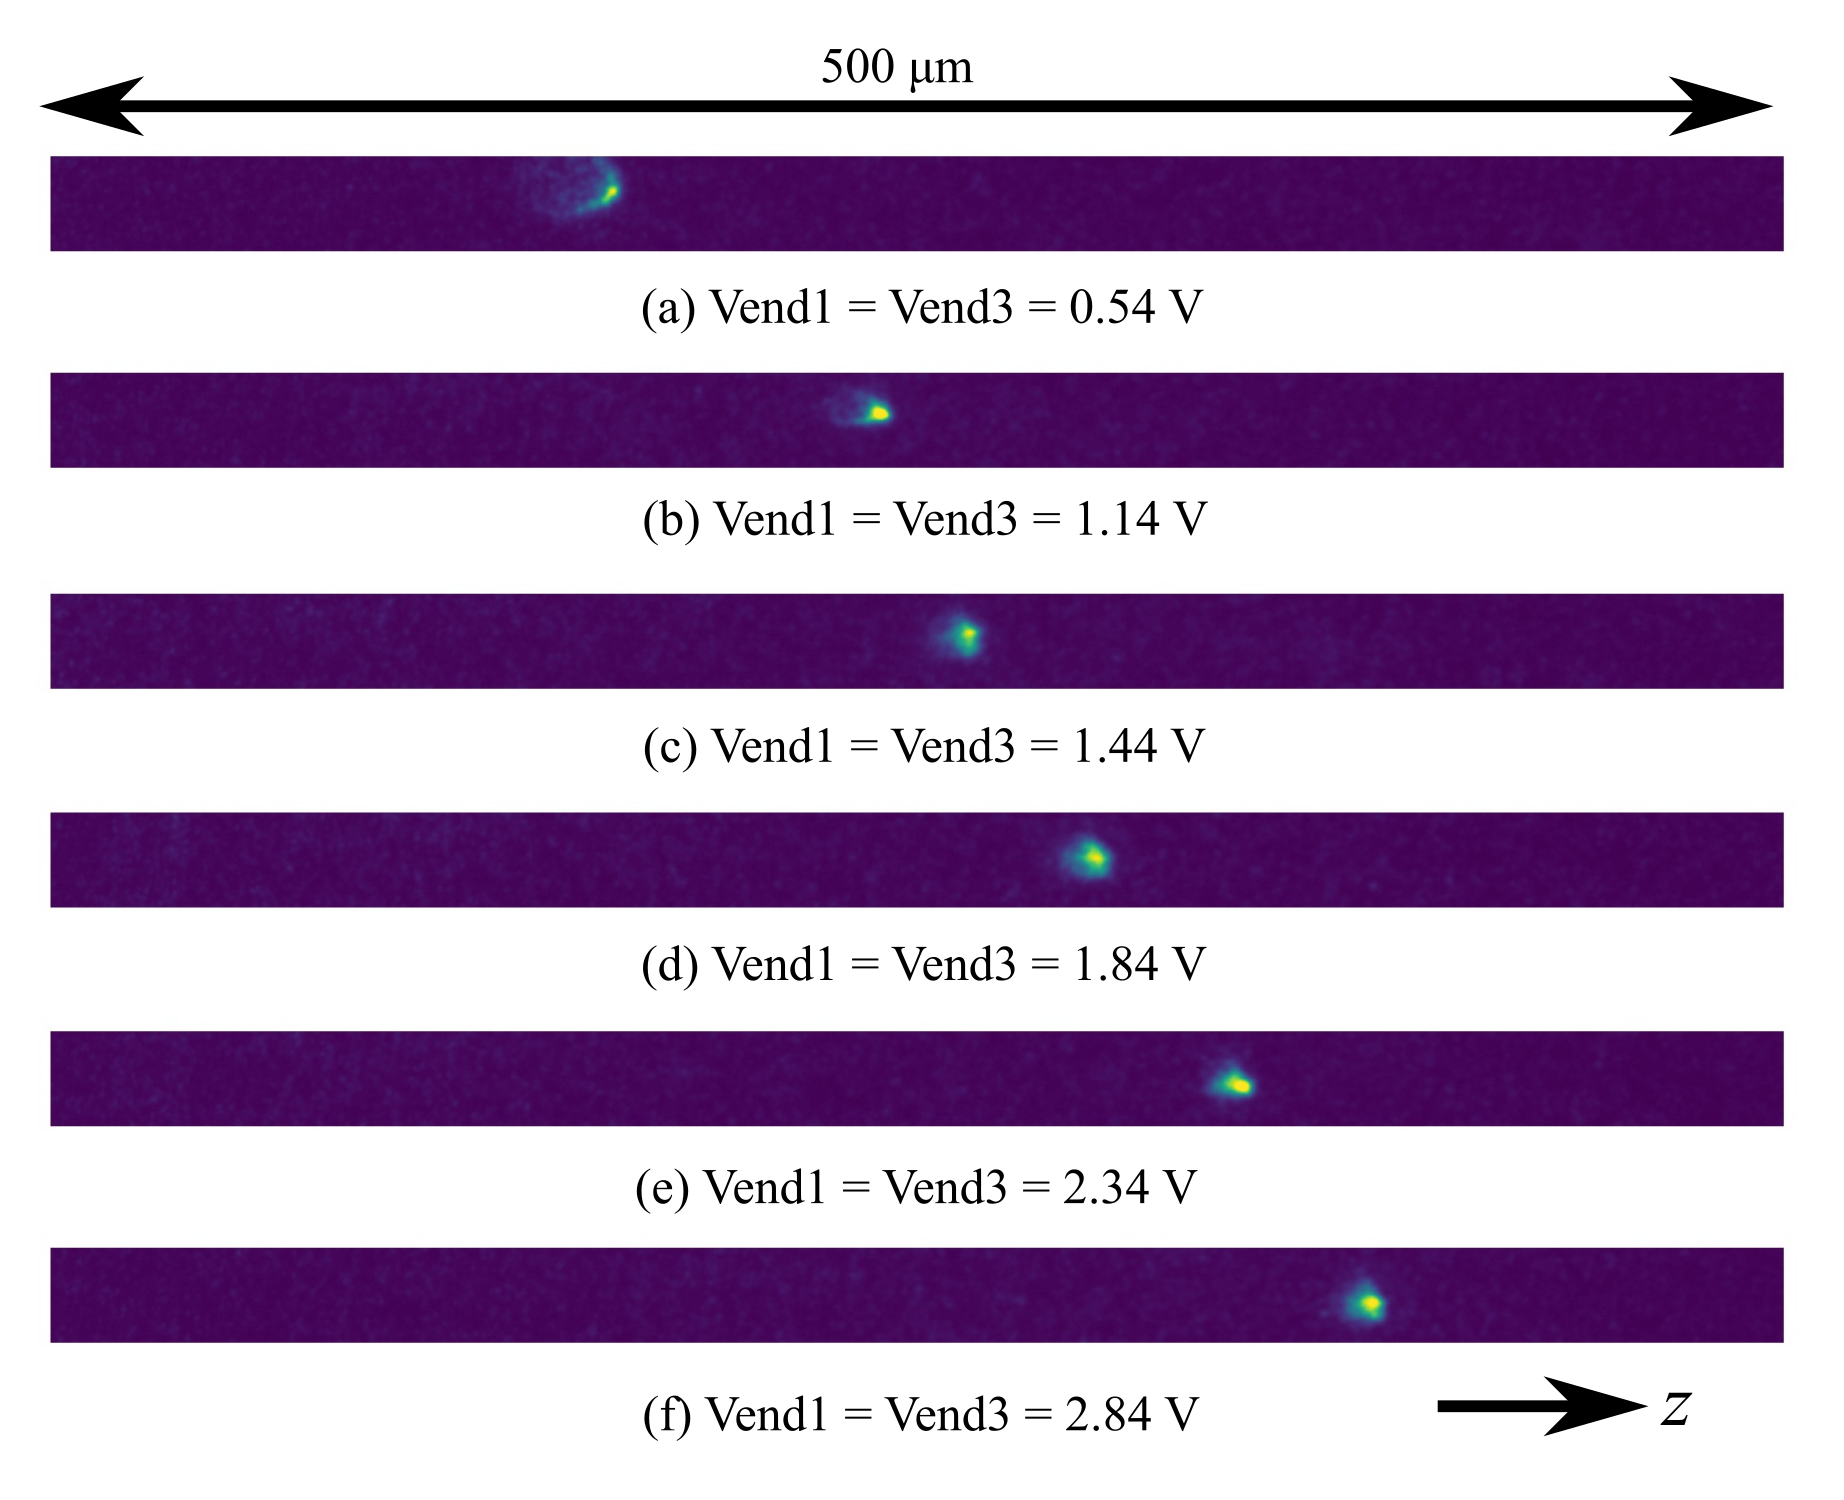
\includegraphics[scale = 0.7]{./results/figure/displacement_End_Odd.png}
		\caption{$V_{\rm End1}, V_{\rm End3} = 0.54{\rm \ (a)}, \ 1.14{\rm \ (b)}, \ 1.44{\rm \ (c)}, \ 1.84{\rm \ (d)}, \ 2.34{\rm \ (e)}, \ 2.84{\rm \ (f)} \ {\rm V}$のときのイオン捕獲画像}
		\label{fig:displacement_End13}
	\end{center}
\end{figure}

\Fig{displacement_End13}より,End1とEnd3に印加するdc電圧が大きいとイオンの捕獲位置が$+z$方向へ変位し,小さい場合には$-z$方向へ変位することが分かる.\Fig{sim_exp_displacement_End13}に実測値とシミュレーション値の比較したグラフを示す.

\begin{figure}[h]
	\begin{center}
		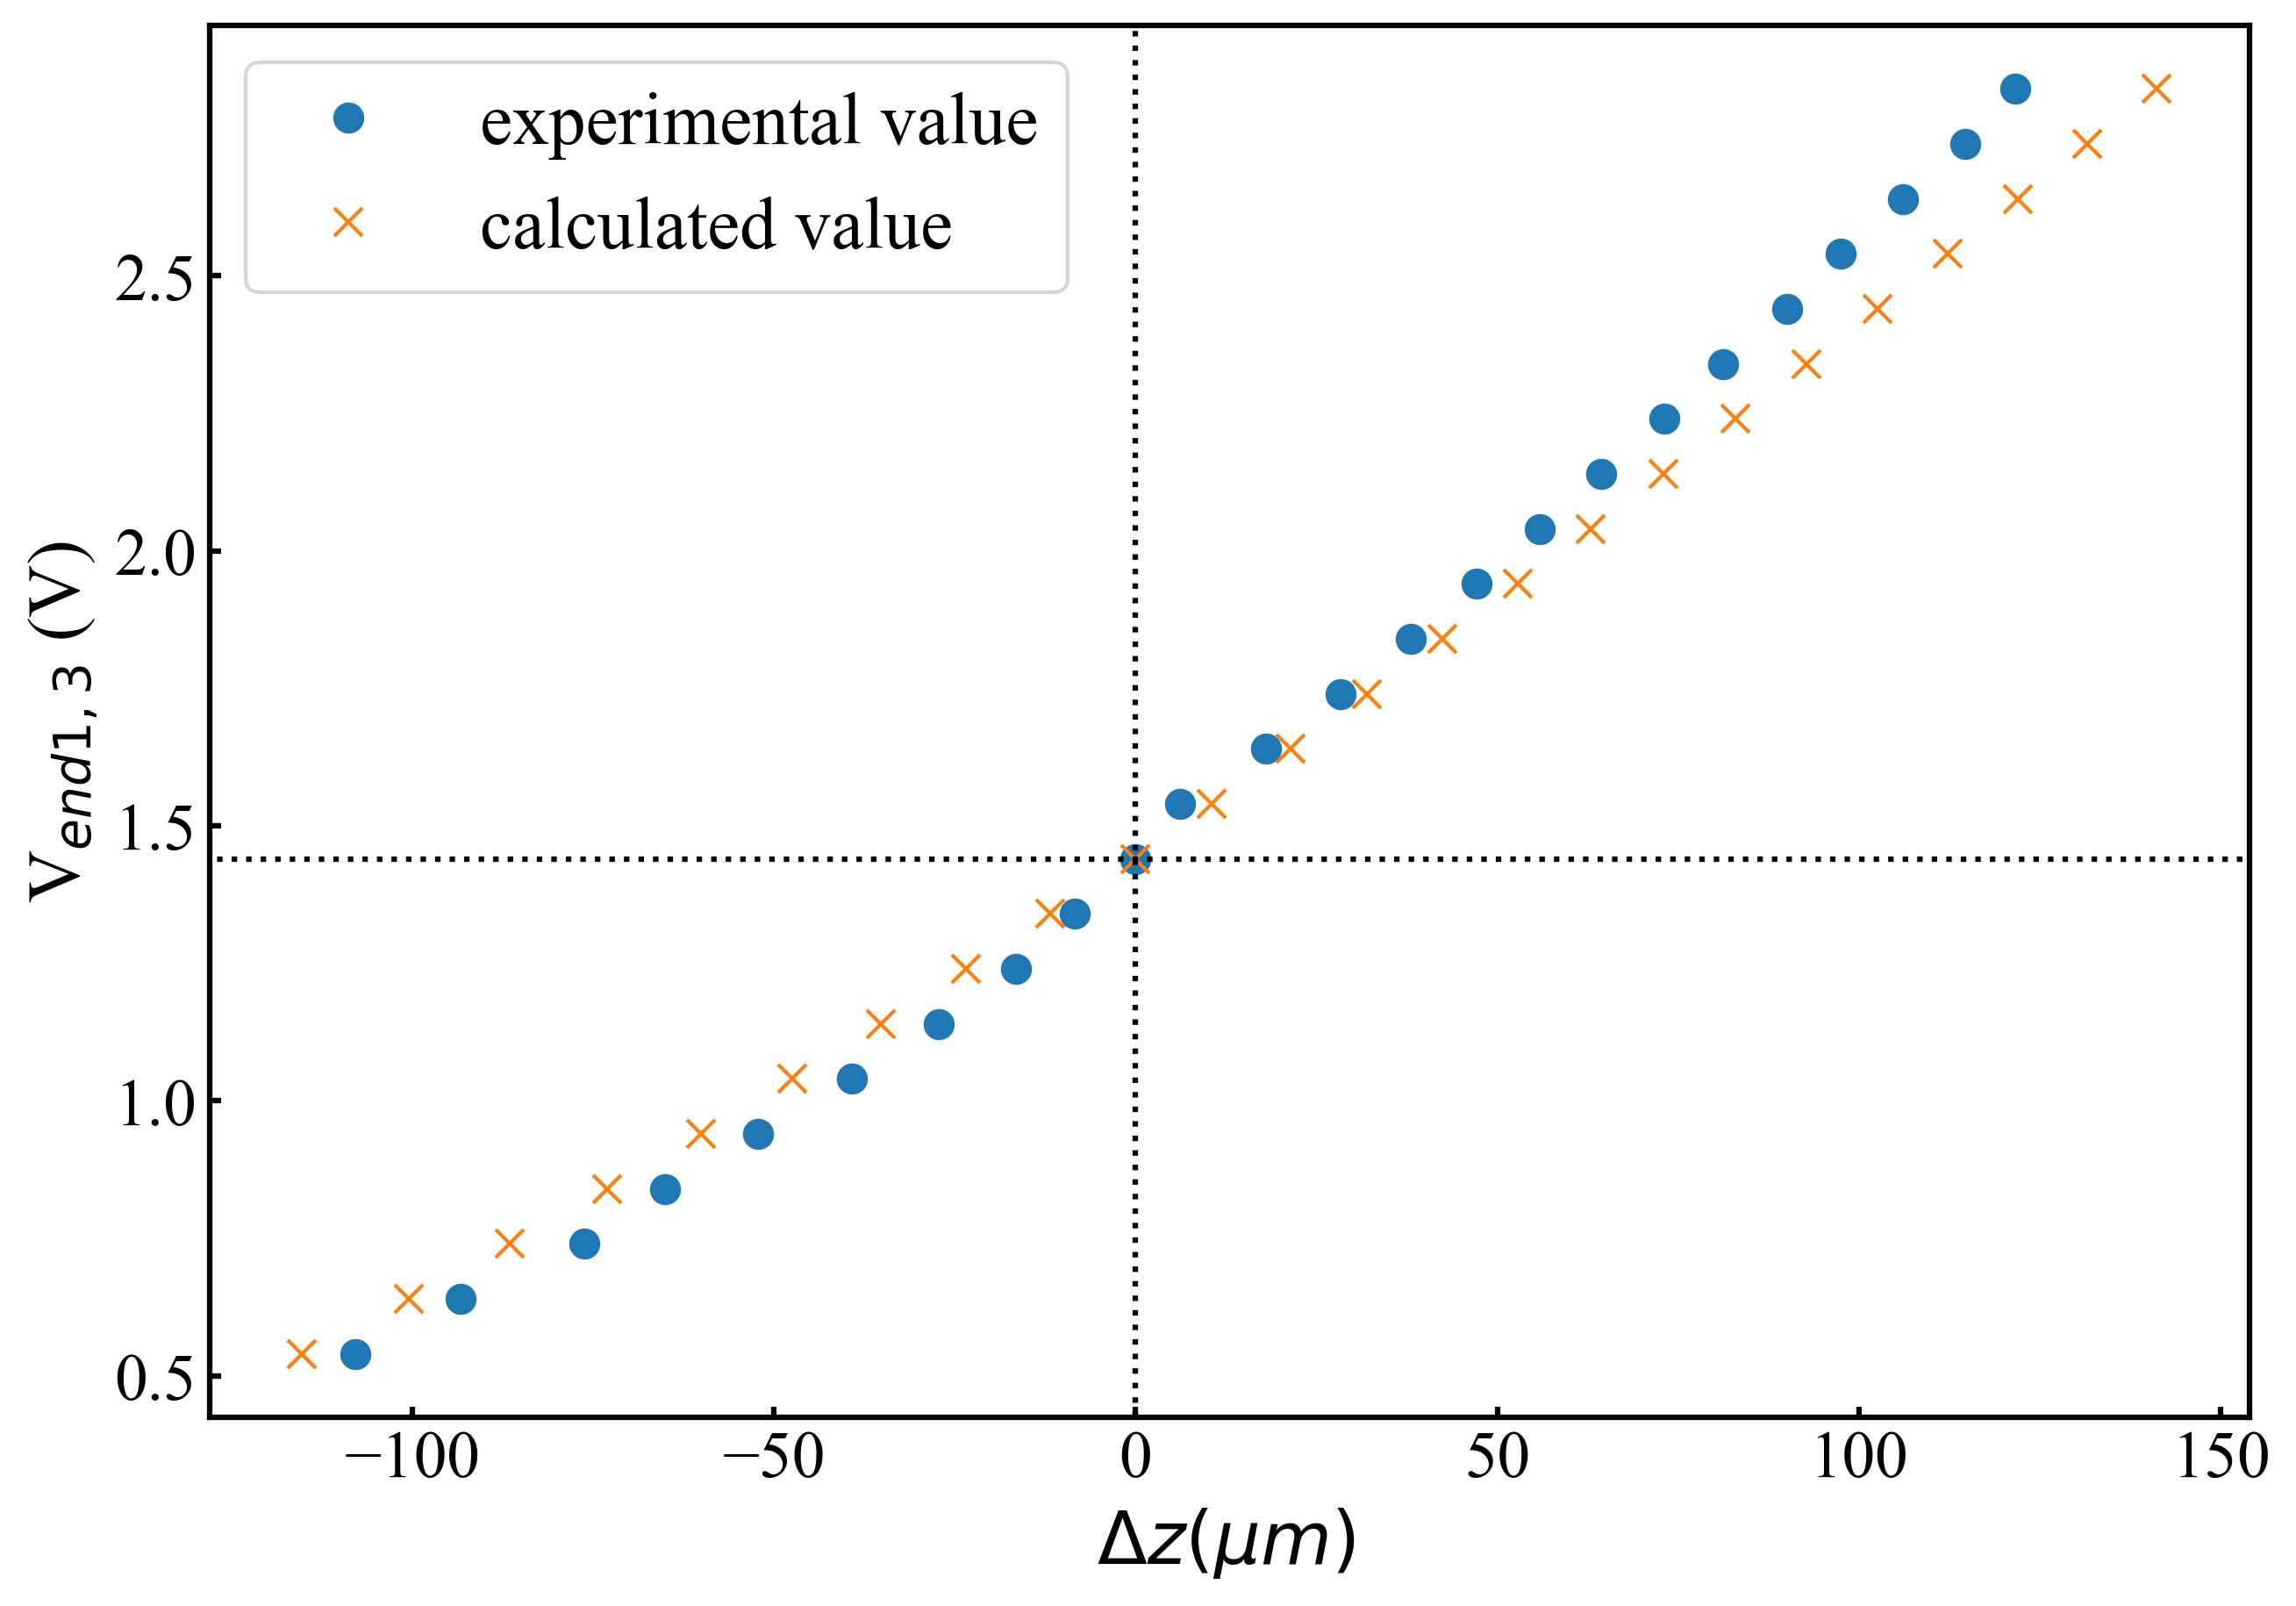
\includegraphics[width = 0.7\linewidth]{./results/figure/out_V13.jpg}
		\caption{\Tb{dc_string}の条件にて${\rm V}_{\rm End1}$と${\rm V}_{\rm End3}$の値を$0.54 \sim 2.84$Vまで0.1Vずつ変化させたときのイオン捕獲位置の変位の実測値とシミュレーション値との比較}
		\label{fig:sim_exp_displacement_End13}
	\end{center}
\end{figure}

End2とEnd4の電極に印加するdc電圧の変化に対するイオン捕獲位置の変位についても同様の実験を行った.実測値とシミュレーション値との比較を\Fig{sim_exp_displacement_End24}に示す.

\begin{figure}[h]
	\begin{center}
		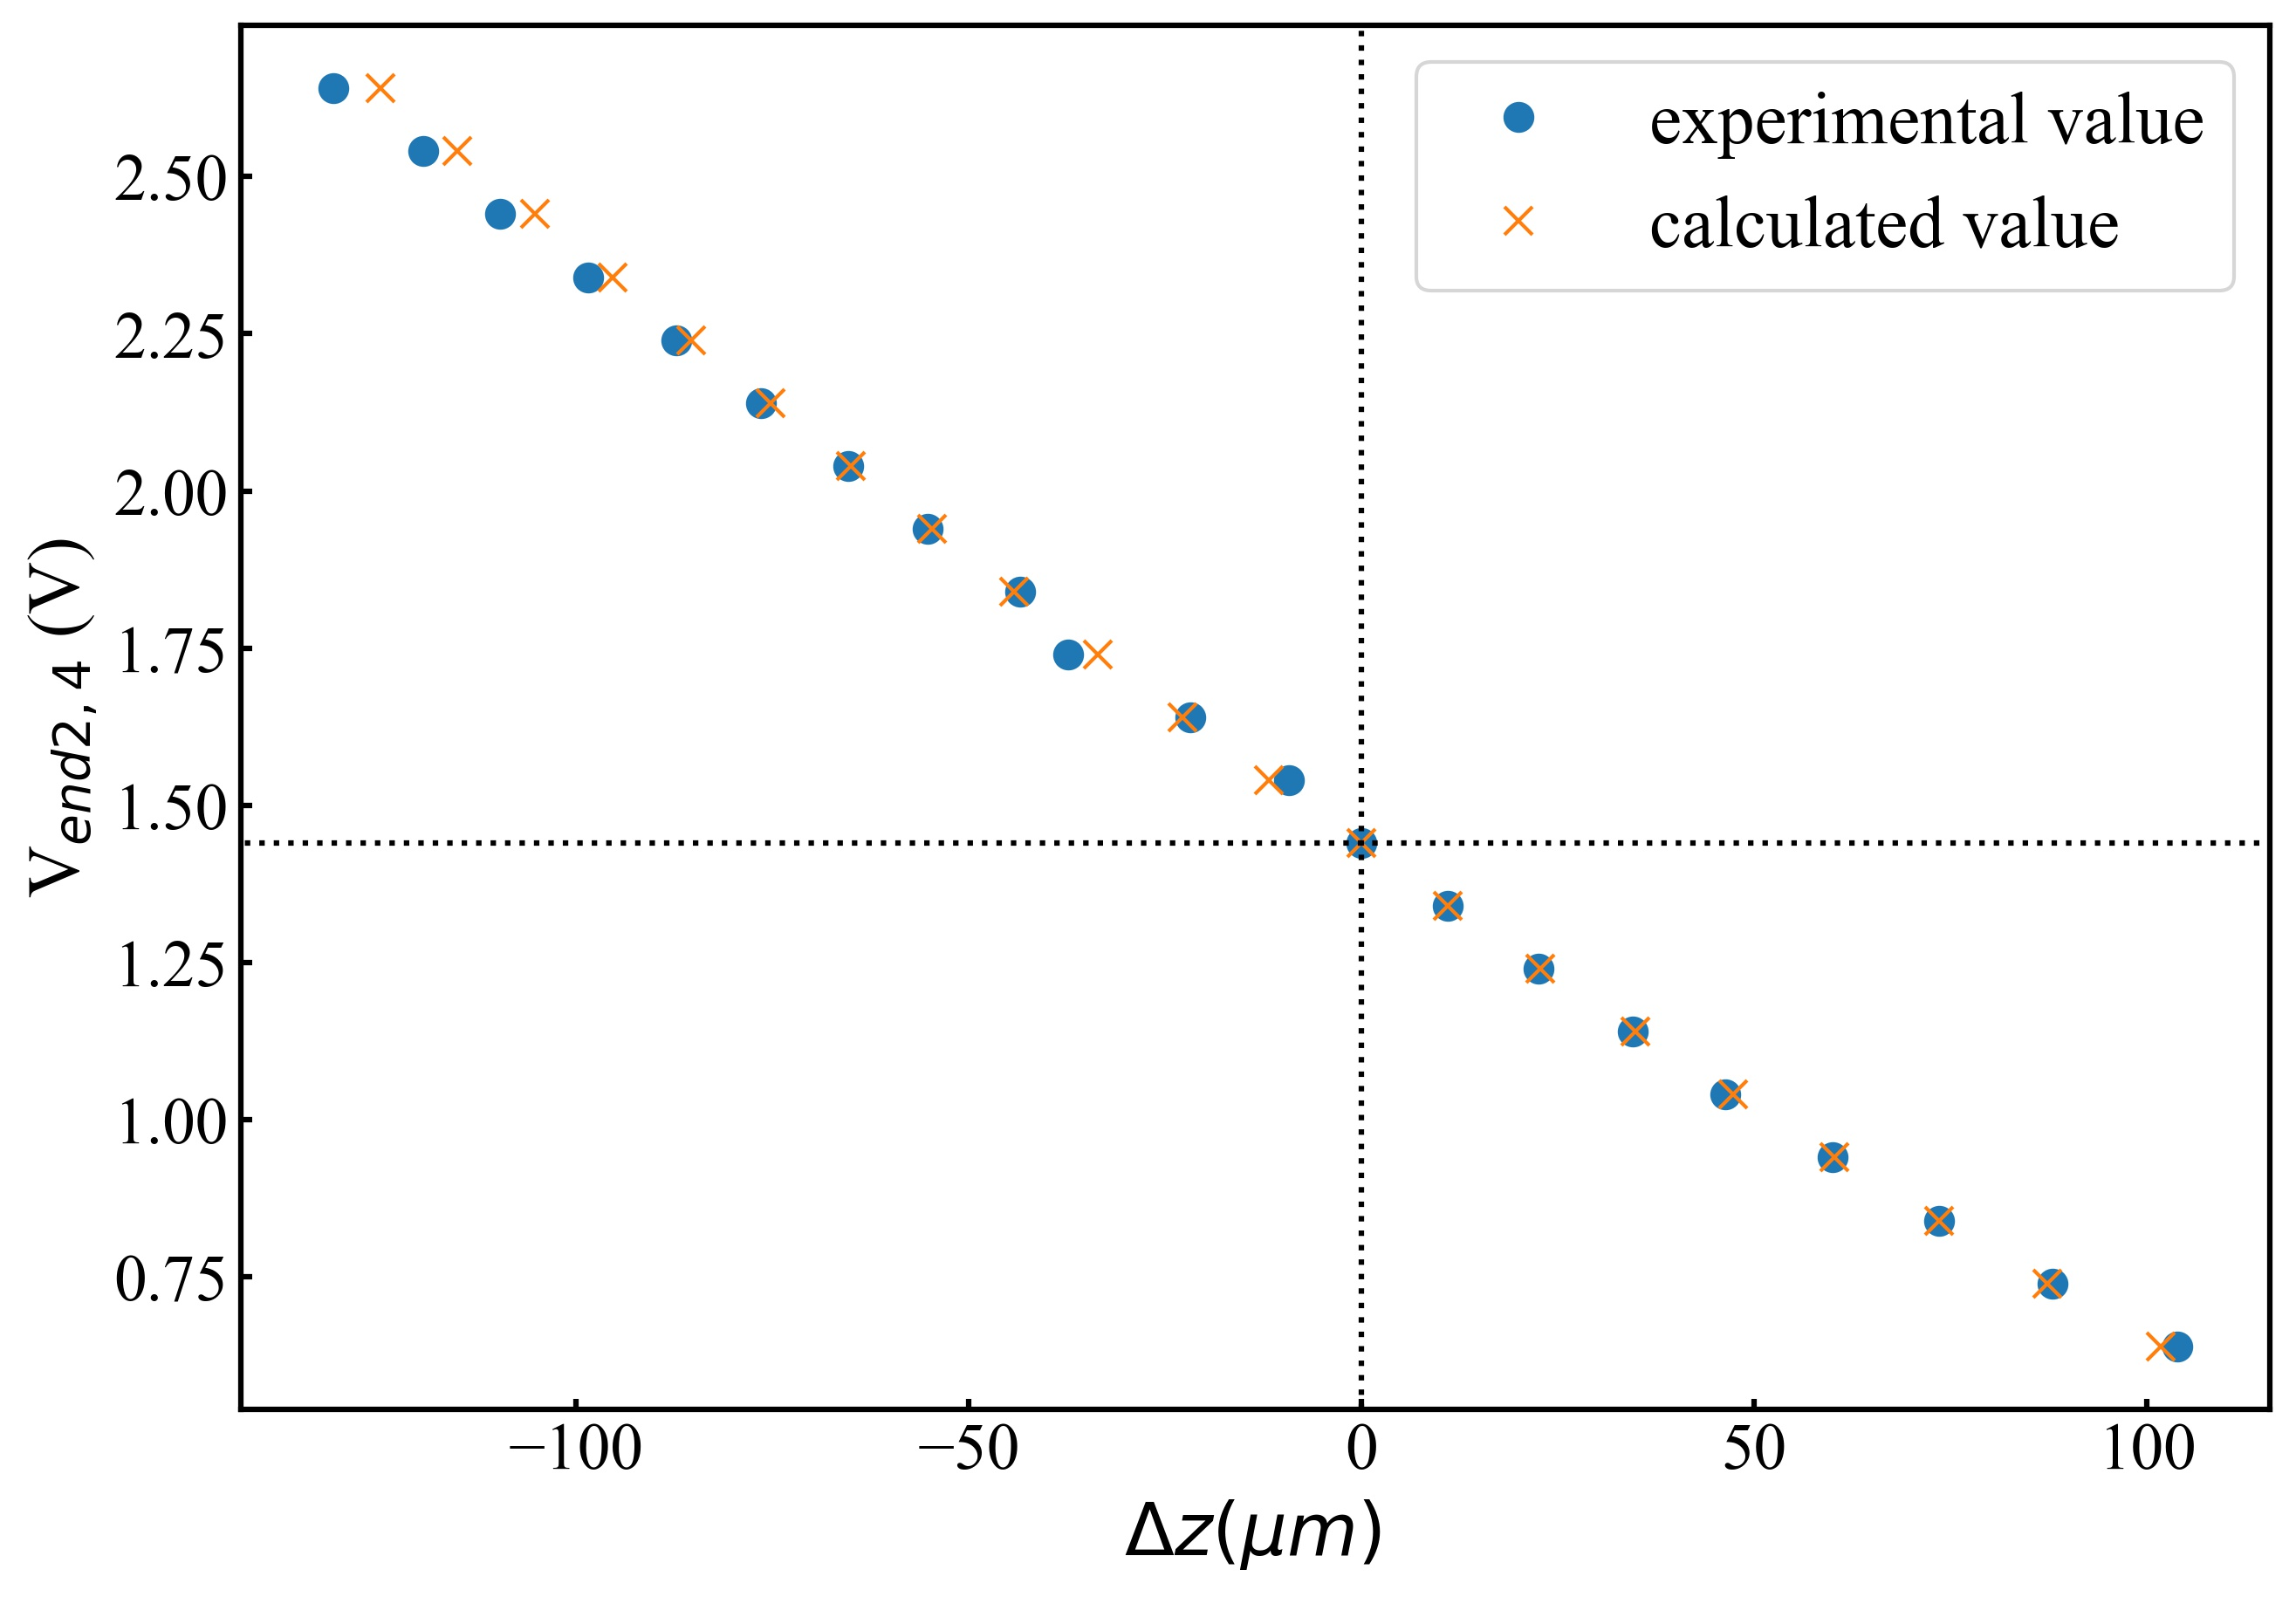
\includegraphics[width = 0.7\linewidth]{./results/figure/out_V24.jpg}
		\caption{\Tb{dc_string}の条件にて${\rm V}_{\rm End2}$と${\rm V}_{\rm End4}$の値を$0.54 \sim 2.84$Vまで0.1Vずつ変化させたときのイオン捕獲位置の変位の実測値とシミュレーション値との比較}
			\label{fig:sim_exp_displacement_End24}
	\end{center}
\end{figure}
\Fig{sim_exp_displacement_End24}より,End2とEnd4に印加するdc電圧が小さい場合に$+z$方向へイオン捕獲位置が変位し,大きい場合に$-z$方向へ変位することが確認できた.
\subsection{永年周波数のdc電圧依存性}

\begin{figure}[h]
	\begin{center}
		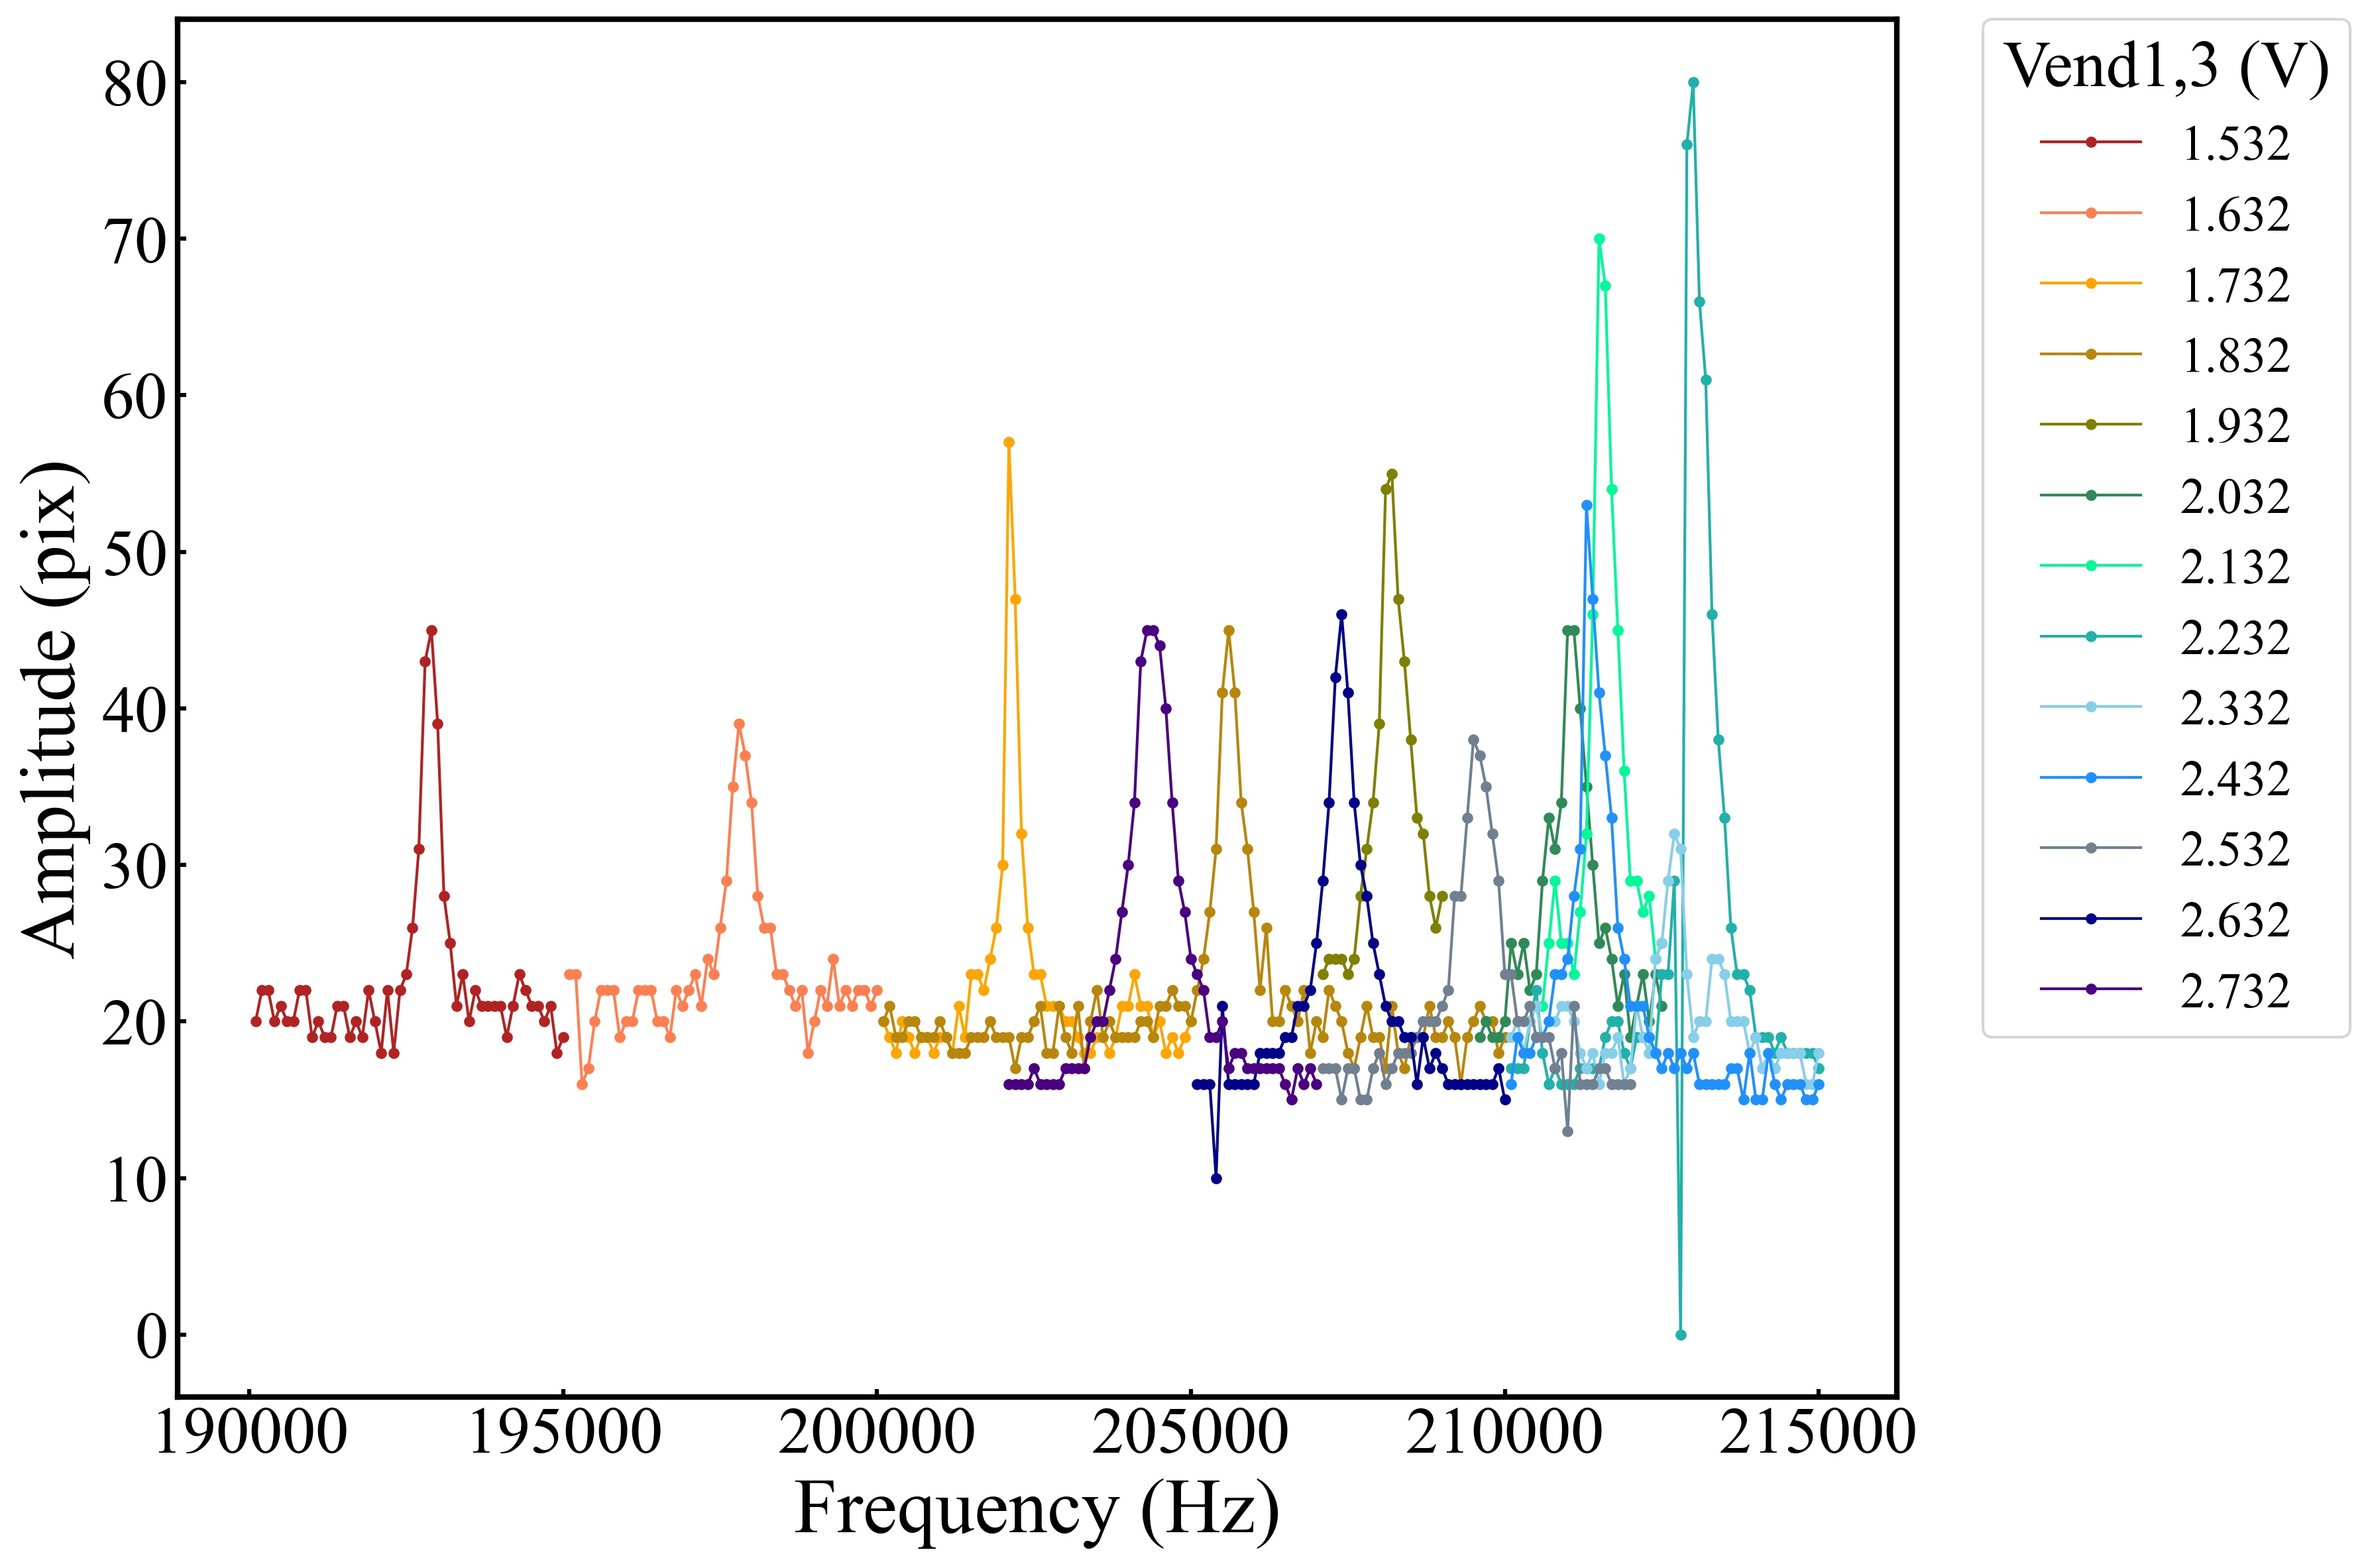
\includegraphics[width = 0.7\linewidth]{./results/figure/end13-SecFreq.jpg}
		\caption{$V_{\rm End1}$と$V_{\rm End3}$を変化させたときの永年周波数の測定結果}
		\label{fig:end13_MeasSec}
	\end{center}
\end{figure}

\begin{figure}[h]
	\begin{center}
		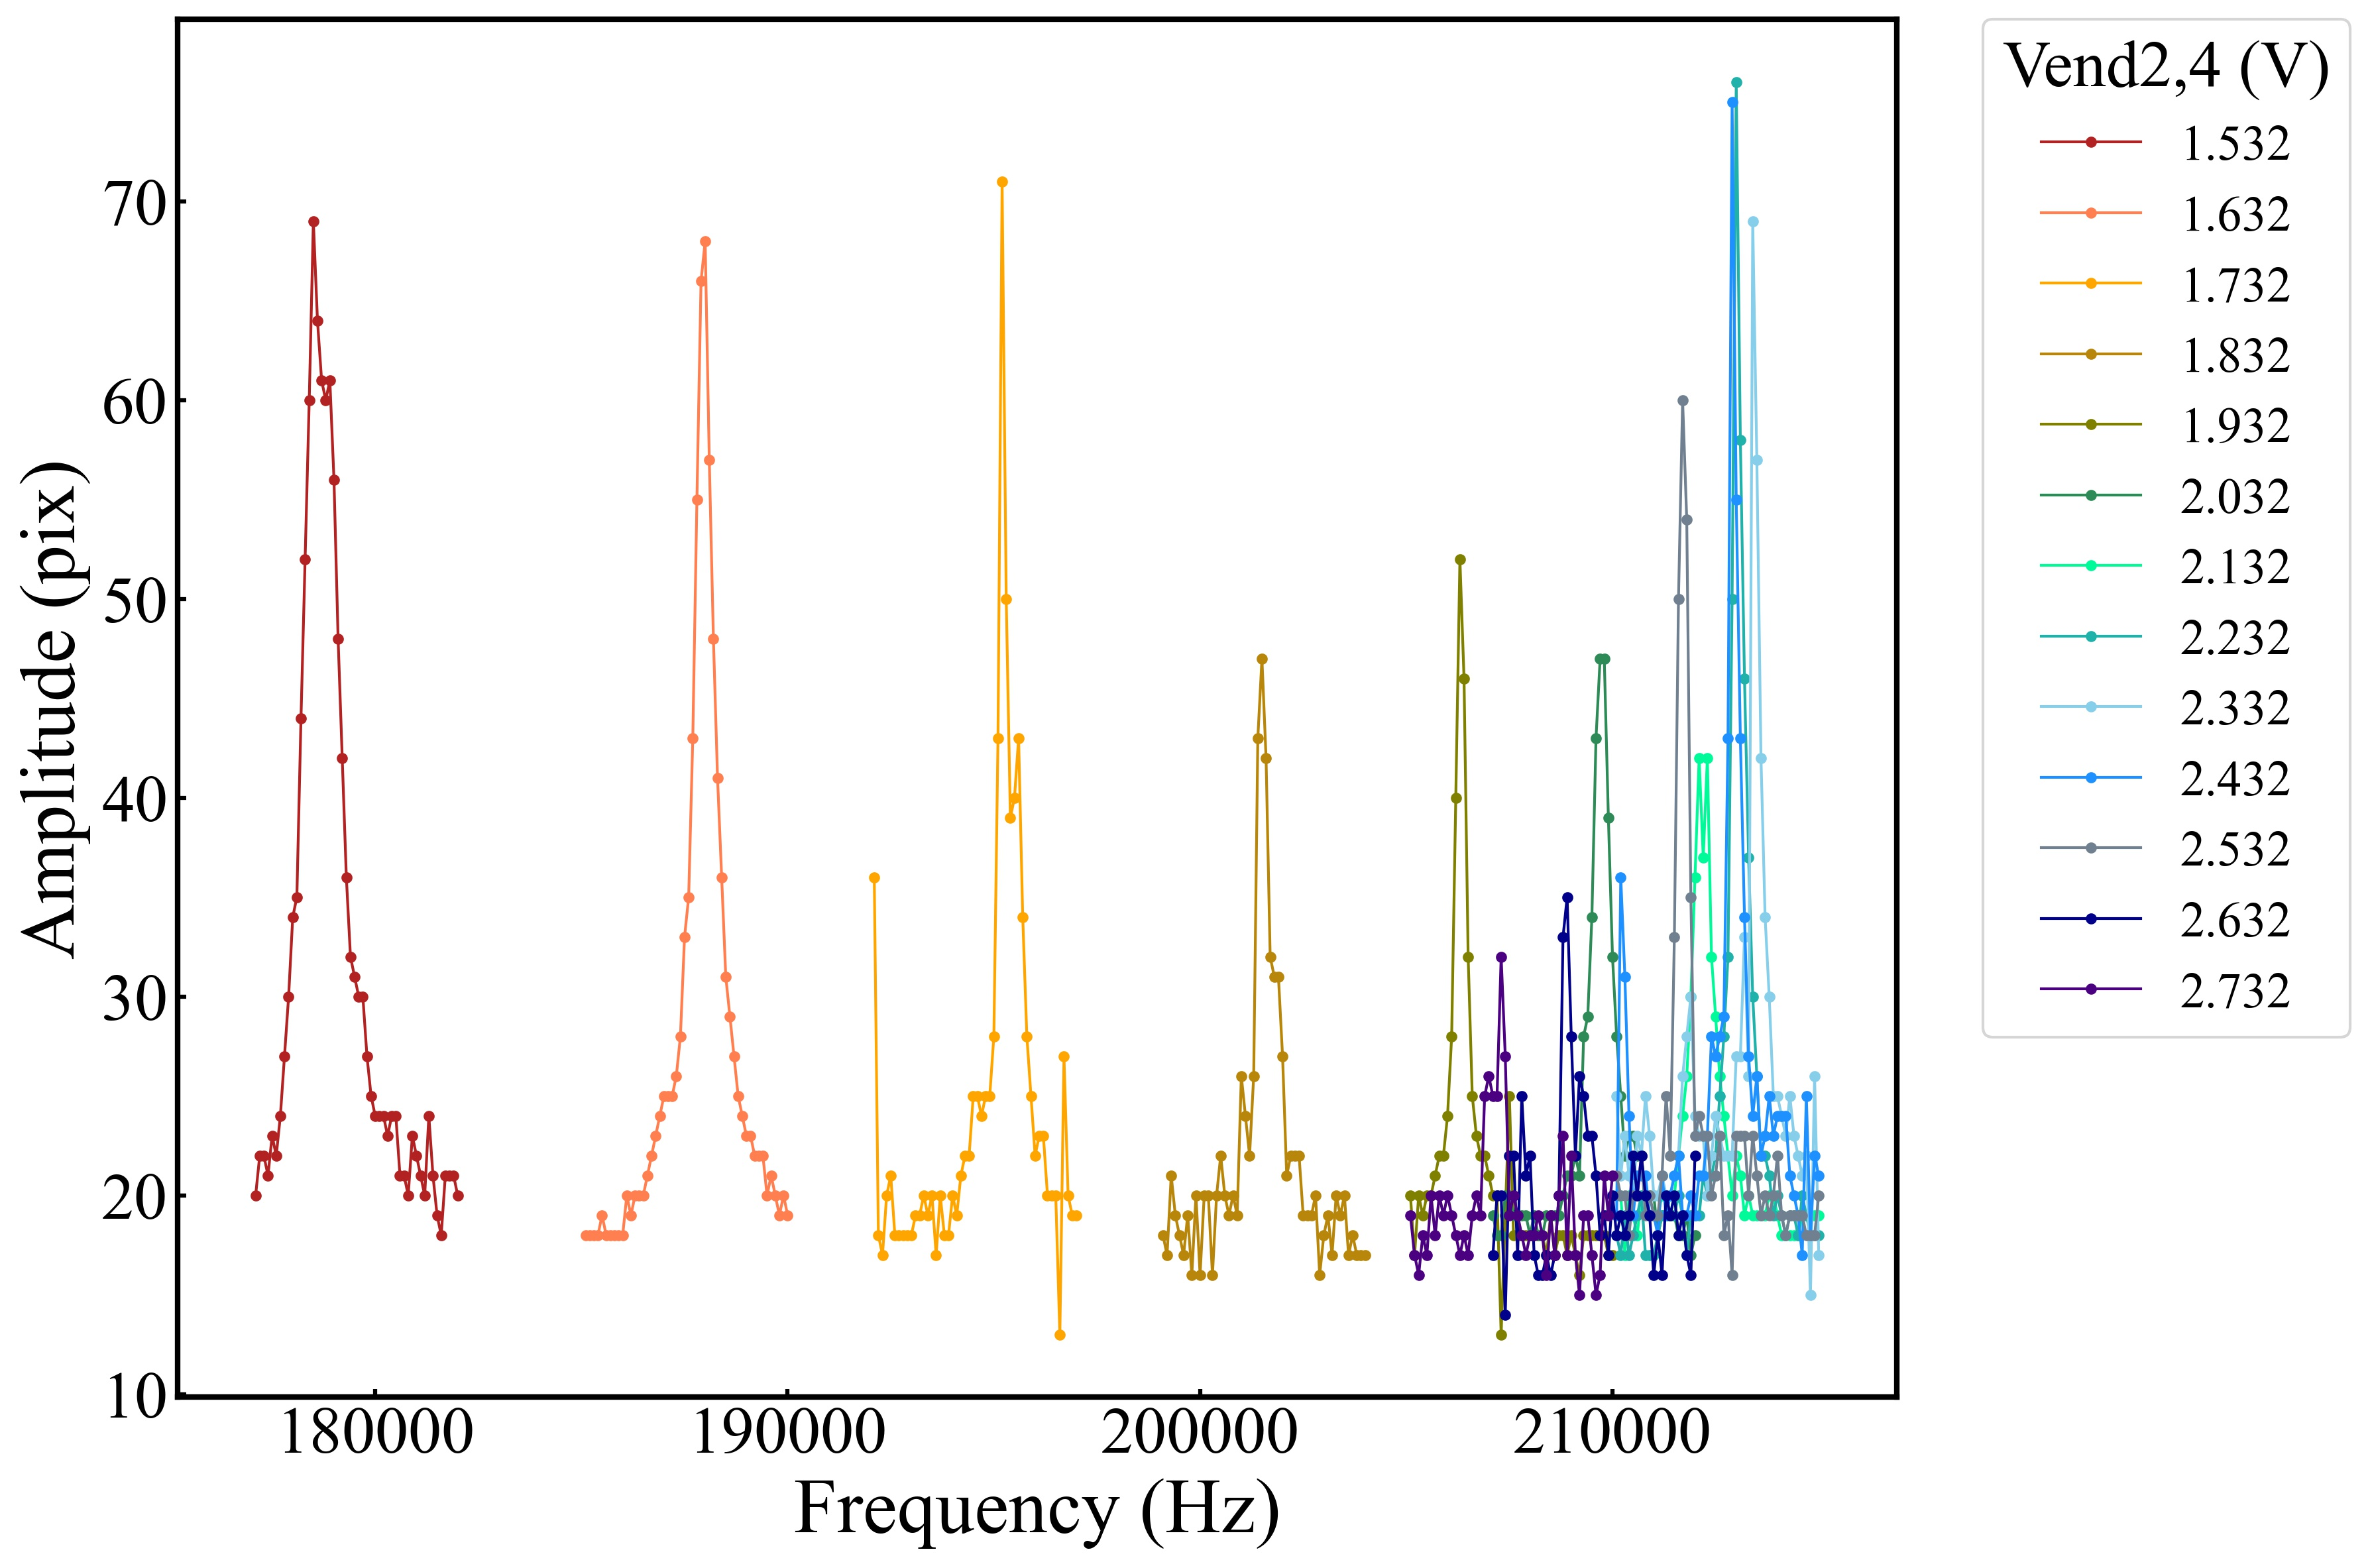
\includegraphics[width = 0.7\linewidth]{./results/figure/end24-SecFreq.jpg}
		\caption{$V_{\rm End2}$と$V_{\rm End4}$を変化させたときの永年周波数の測定結果}
		\label{fig:end24_MeasSec}
	\end{center}
\end{figure}

\begin{figure}[h]
	\begin{center}
		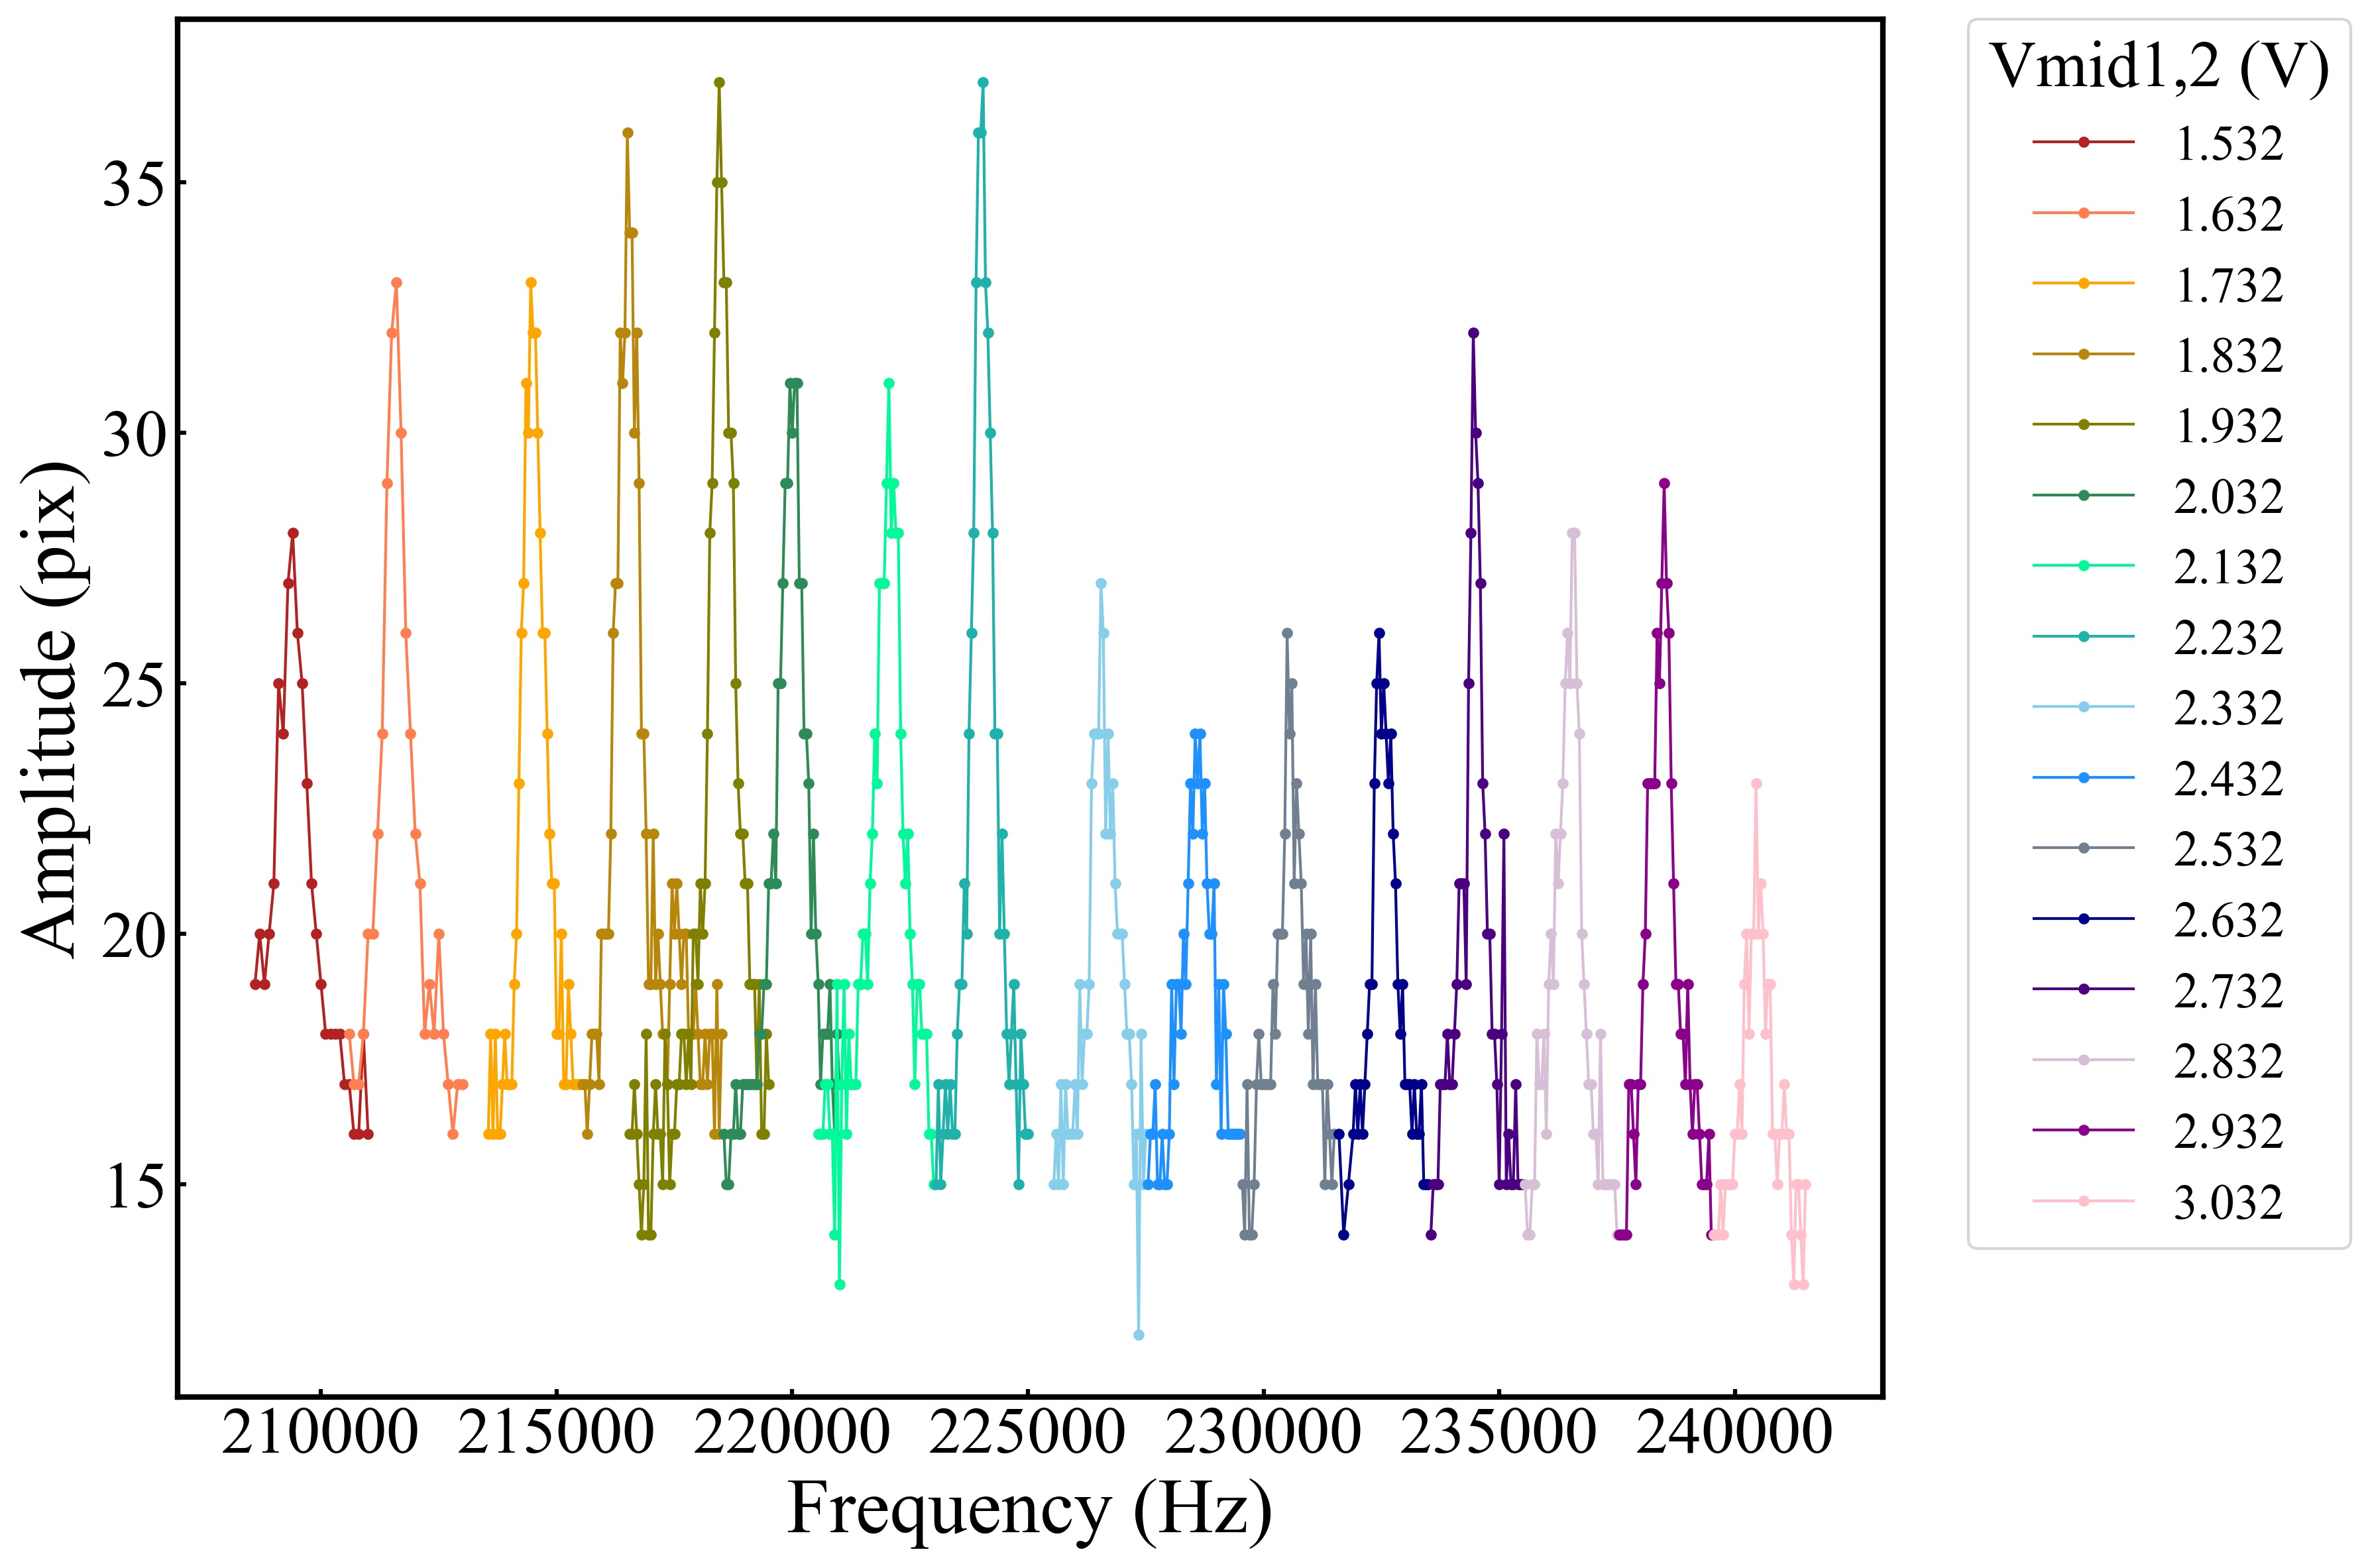
\includegraphics[width = 0.7\linewidth]{./results/figure/mid-SecFreq.jpg}
		\caption{$V_{\rm Middle1}$と$V_{\rm Middle2}$を変化させたときの永年周波数の測定結果}
		\label{fig:mid_MeasSec}
	\end{center}
\end{figure}

\section{二列配列イオン}
\subsection{イオン列間距離dと比率Rとの関係}
\subsection{永年周波数の測定結果}